\chapter{Strength in Numbers}
\label{les:15}

\begin{chapquote}{Lewis Carroll, \textit{Alice im Wunderland}}
\enquote{Mal sehen: Viermal fünf ist zwölf, und viermal sechs ist dreizehn, und
viermal sieben ist vierzehn – oh je! Auf diese Weise komme ich ja nie bis
Zwanzig!}
\end{chapquote}

Zahlen sind ein wesentlicher Bestandteil unseres alltäglichen Lebens. Die
meisten von uns sind jedoch nicht recht gut mit großen Zahlen vertraut. Die
größten Zahlen denen wir im täglichen Leben begegnen, liegen in der
Größenordnung von Millionen, Milliarden oder Billionen. Wir können über
Millionen von Menschen in Armut oder Milliarden von Dollar die für die
Rettungsschirme für Banken ausgegeben werden oder gar über Trillionen von
Staatsschulden lesen. Auch wenn es schwer ist diese Schlagzeilen zu
interpretieren, können wir Zahlen dieser Größenordnung gewissermaßen einordnen.

Obwohl wir mit Milliarden und Billionen noch etwas anfangen können, beginnt
unsere Intuition bereits bei Zahlen der Größenordnung Milliarden zu versagen.
Hast du eine Ahnung, wie lange du warten müsstest bis eine Million / Milliarden
/ Billionen Sekunden vergehen? Wenn du nur ein bisschen wie ich bist, wärst du
jetzt verloren ohne die Zahlen genauer runterzubrechen.

Betrachten wir das Beispiel: Der Unterschied ist eine Erhöhung um drei
Zehnerpotenzen: $10^6$, $10^9$, $10^{12}$. In Sekunden zu denken bringt uns
nicht weiter also lass uns das in etwas übersetzen das wir verstehen:

\begin{itemize}
  \item $10^6$: Eine Million Sekunden war vor $1 1/2$ Wochen.
  \item $10^9$: Eine Milliarde Sekunden war vor fast 32 Jahren.
  \item $10^{12}$: Vor einer Billion Sekunden war Manhattan noch von einer
  dicken Eisschicht bedeckt.\footnote{Eine Billion Sekunden ($10^{12}$)
  entspricht $31.710$ Jahren. Das letzte Glazial setzte vor etwa 115.000 Jahren
  ein und endete vor etwa 11.700 Jahren.~\cite{wiki:LGM}}
\end{itemize}

\begin{figure}
  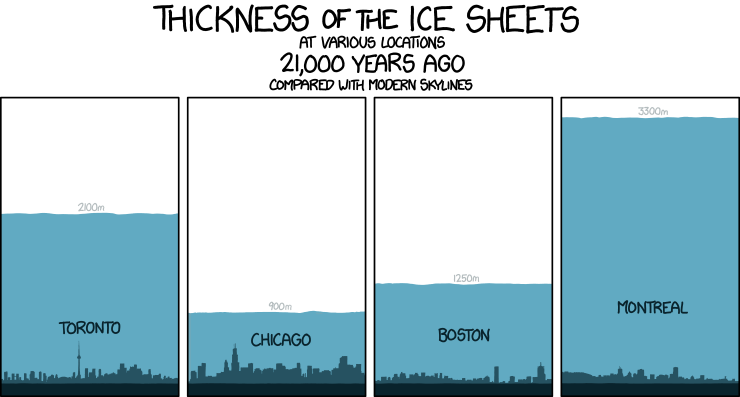
\includegraphics{assets/images/xkcd-1225.png}
  \caption{Dicke der Eisschichten vor ungefähr einer Billion Sekunden. Quelle: xkcd 1225}
  \label{fig:xkcd-1225}
\end{figure}

Sobald wir in den Bereich der modernen Kryptographie eintreten, versagt unsere
Intuition katastrophal. Bitcoin wurde um große Zahlen herum aufgebaut. Alles mit
der Tatsache, dass es praktisch unmöglich ist diese zu erraten. Die Zahlen sind
weitaus größer als alles was uns im Alltag begegnen könnte. Viele Zehnerpotenzen
größer. Zu verstehen wie groß diese Zahlen wirklich sind, ist entscheidend für
das Verständnis von Bitcoin als großem Ganzen.

Nehmen wir SHA-256\footnote{SHA-256 ist Teil von SHA-2, eine Gruppe von
verschiedenen kryptologischen Hashfunktionen welche von der NSA entwickelt
wurde.~\cite{wiki:sha2}}, eine der in Bitcoin verwendeten
Hashfunktionen\footnote{Bitcoin verwendet SHA-256 als
Block-Hashing-Algorithmus.~\cite{btcwiki:block-hashing}} als konkretes Beispiel.
Es liegt in der Natur der Sache, bei 256 Bits an
\enquote{Zweihundertsechsundfünzig} zu denken, was an sich ja keine große Zahl
ist. Die Zahl in SHA-256 spricht jedoch von Potenzen -- etwas womit unser Gehirn
eben nicht sonderlich gut klar kommt.

Während die Länge der Bits eine bequeme Metrik ist, geht die wahre Bedeutung der
256-Bit-Sicherheit bei der Übersetzung verloren. Ähnlich wie bei den oben
genannten Millionen ($10^6$) und Milliarden ($10^9$) spricht die Zahl in SHA-256
von Größenordnungen ($2^{256}$).

Also, wie stark ist SHA-256 genau?

\begin{quotation}\begin{samepage}
\enquote{SHA-256 ist sehr stark. Es ist nicht wie der nächste Schritt von MD5 zu
SHA1. Es kann mehrere Jahrzehnte andauern, es sei denn es gibt einen massiven
technologischen Durchbruch.}
\begin{flushright} -- Satoshi Nakamoto\footnote{Satoshi Nakamoto, in einer
Antwort zu Fragen über SHA-256 Kollisionen. \cite{satoshi-sha256}}
\end{flushright}\end{samepage}\end{quotation}

Ausgeschrieben ergibt $2^{256}$ folgende Zahl:

\begin{quotation}\begin{samepage}
    115 quattuorvigintillion 792 trevigintillion 89 duovigintillion 237
    unvigintillion 316 vigintillion 195 novemdecillion 423 octodecillion 570
    septendecillion 985 sexdecillion 8 quindecillion 687 quattuordecillion 907
    tredecillion 853 duodecillion 269 undecillion 984 decillion 665 nonillion
    640 octillion 564 septillion 39 sextillion 457 quintillion 584 quadrillion 7
    trillion 913 billion 129 million 639 thousand 936.
\end{samepage}\end{quotation}

That's a lot of nonillions! Wrapping your head around this number is
pretty much impossible. There is nothing in the physical universe to
compare it to. It is far larger than the number of atoms in the
observable universe. The human brain simply isn't made to make sense of
it.

\newpage

One of the best visualizations of the true strength of SHA-256 is a video by
Grant Sanderson. Aptly named \textit{\enquote{How secure is 256 bit
security?}}\footnote{Watch the video at \url{https://youtu.be/S9JGmA5_unY}} it
beautifully shows how large a 256-bit space is. Do yourself a favor and take the
five minutes to watch it. As all other \textit{3Blue1Brown} videos it is not
only fascinating but also exceptionally well made. Warning: You might fall down
a math rabbit hole.

\begin{figure}
  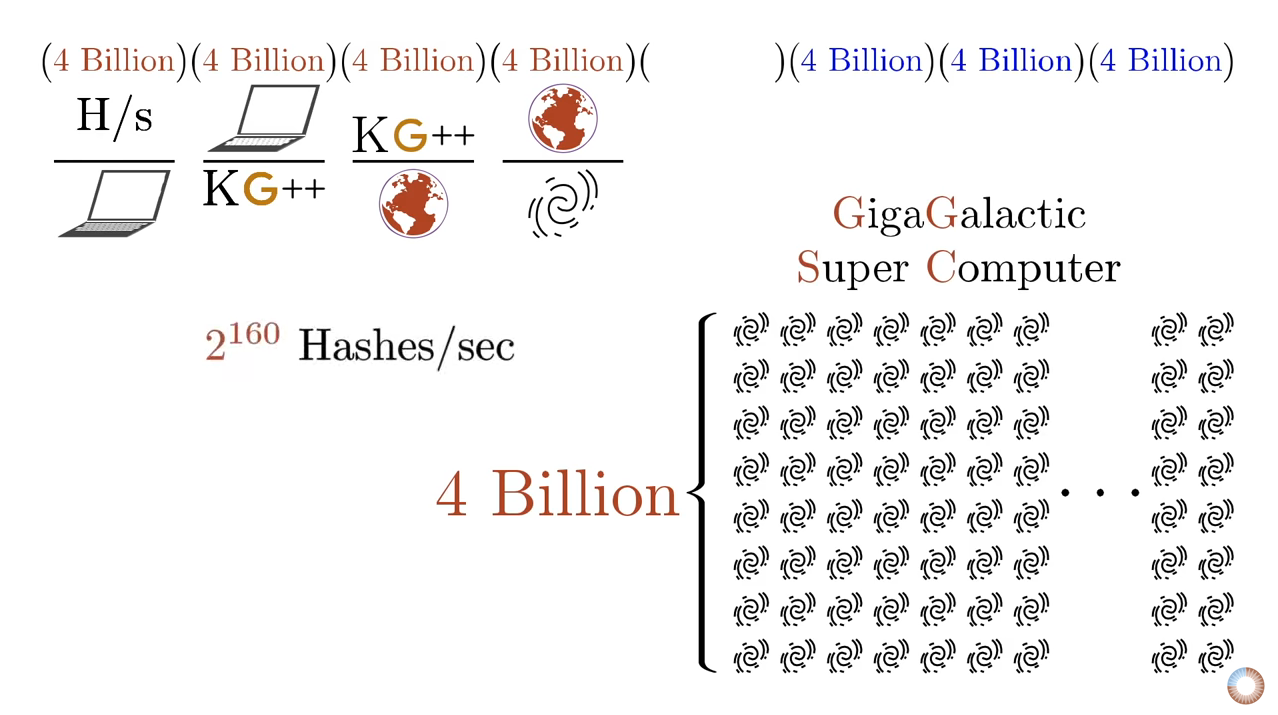
\includegraphics{assets/images/youtube-vid-inverted.png}
  \caption{Illustration of SHA-256 security. Original graphic by Grant Sanderson aka 3Blue1Brown.}
  \label{fig:youtube-vid-inverted}
\end{figure}

Bruce Schneier~\cite{web:schneier} used the physical limits of computation to put this
number into perspective: even if we could build an optimal computer,
which would use any provided energy to flip bits perfectly~\cite{wiki:landauer}, build a
Dyson sphere\footnote{A Dyson sphere is a hypothetical megastructure that completely encompasses a star and captures a large percentage of its power output.~\cite{wiki:dyson}} around our sun, and let it run for 100 billion billion
years, we would still only have a $25\%$ chance to find a needle in a
256-bit haystack.

\begin{quotation}\begin{samepage}
\enquote{These numbers have nothing to do with the technology of the devices;
they are the maximums that thermodynamics will allow. And they
strongly imply that brute-force attacks against 256-bit keys will be
infeasible until computers are built from something other than matter
and occupy something other than space.}
\begin{flushright} -- Bruce Schneier\footnote{Bruce Schneier, \textit{Applied Cryptography} \cite{bruce-schneier}}
\end{flushright}\end{samepage}\end{quotation}


It is hard to overstate the profoundness of this. Strong cryptography
inverts the power-balance of the physical world we are so used to.
Unbreakable things do not exist in the real world. Apply enough force,
and you will be able to open any door, box, or treasure chest.

Bitcoin's treasure chest is very different. It is secured by strong
cryptography, which does not give way to brute force. And as long as the
underlying mathematical assumptions hold, brute force is all we have.
Granted, there is also the option of a global \$5 wrench attack (Figure~\ref{fig:xkcd-538})
But torture won't work for all bitcoin addresses, and the cryptographic
walls of bitcoin will defeat brute force attacks. Even if you come at it
with the force of a thousand suns. Literally.

\begin{figure}
  \centering
  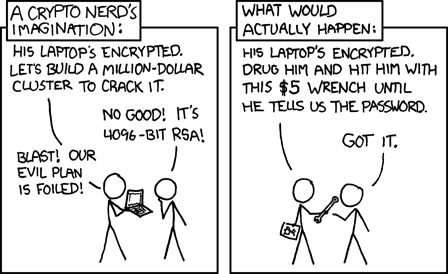
\includegraphics[width=8cm]{assets/images/xkcd-538.png}
  \caption{\$5 wrench attack. Source: xkcd 538}
  \label{fig:xkcd-538}
\end{figure}

This fact and its implications were poignantly summarized in the call
to cryptographic arms: \textit{\enquote{No amount of coercive force will ever solve
a math problem.}}

\begin{quotation}\begin{samepage}
\enquote{It isn't obvious that the world had to work this way. But somehow the
universe smiles on encryption.}
\begin{flushright} -- Julian Assange\footnote{Julian Assange, \textit{A Call to Cryptographic Arms} \cite{call-to-cryptographic-arms}}
\end{flushright}\end{samepage}\end{quotation}

Nobody yet knows for sure if the universe's smile is genuine or not. It
is possible that our assumption of mathematical asymmetries is wrong and
we find that P actually equals NP \cite{wiki:pnp}, or we find surprisingly quick
solutions to specific problems \cite{wiki:discrete-log} which we currently assume to be hard.
If that should be the case, cryptography as we know it will cease to
exist, and the implications would most likely change the world beyond
recognition.

\begin{quotation}\begin{samepage}
\enquote{Vires in Numeris} = \enquote{Strength in Numbers}\footnote{\textit{Vires in Numeris} was first proposed as a Bitcoin motto by the bitcointalk user \textit{epii}~\cite{epii}}
\end{samepage}\end{quotation}

\textit{Vires in numeris} is not only a catchy motto used by bitcoiners. The
realization that there is an unfathomable strength to be found in
numbers is a profound one. Understanding this, and the inversion of
existing power balances which it enables changed my view of the world
and the future which lies ahead of us.

One direct result of this is the fact that you don't have to ask anyone
for permission to participate in Bitcoin. There is no page to sign up,
no company in charge, no government agency to send application forms to.
Simply generate a large number and you are pretty much good to go. The
central authority of account creation is mathematics. And God only knows
who is in charge of that.

\begin{figure}
  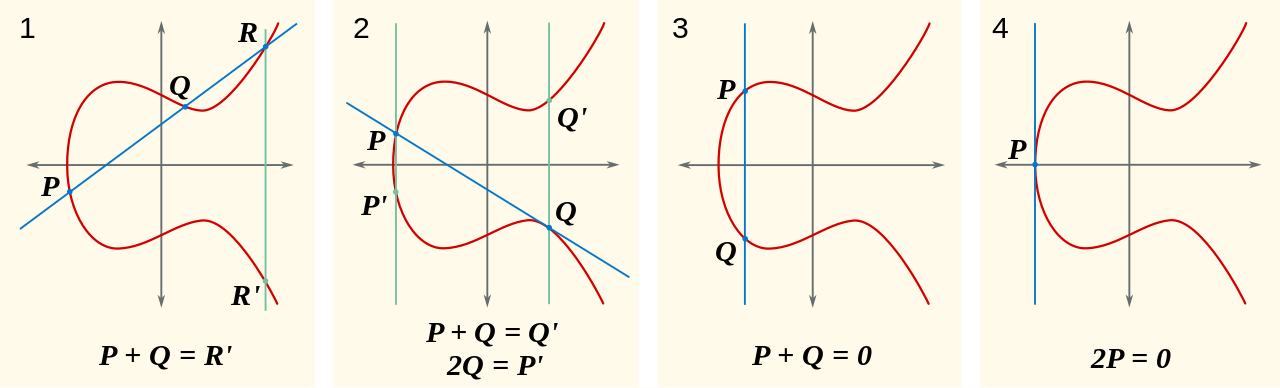
\includegraphics{assets/images/elliptic-curve-examples.png}
  \caption{Elliptic curve examples. Graphic cc-by-sa Emmanuel Boutet.}
  \label{fig:elliptic-curve-examples}
\end{figure}

Bitcoin is built upon our best understanding of reality. While there are
still many open problems in physics, computer science, and mathematics,
we are pretty sure about some things. That there is an asymmetry between
finding solutions and validating the correctness of these solutions is
one such thing. That computation needs energy is another one. In other
words: finding a needle in a haystack is harder than checking if the
pointy thing in your hand is indeed a needle or not. And finding the
needle takes work.

The vastness of Bitcoin's address space is truly mind-boggling. The
number of private keys even more so. It is fascinating how much of our
modern world boils down to the improbability of finding a needle in an
unfathomably large haystack. I am now more aware of this fact than ever.

\paragraph{Bitcoin taught me that there is strength in numbers.}

% ---
%
% #### Down the Rabbit Hole
%
% - [How secure is 256 bit security?]["How secure is 256 bit security?"] by 3Blue1Brown
% - [Block Hashing Algorithm][hash functions] on the Bitcoin Wiki
% - [Last Glacial Maximum][thick layer of ice], [SHA-2][SHA-256], [Dyson Sphere][Dyson sphere], [Landauer's Principle][flip bits perfectly] [P versus NP][P actually equals NP], [Discrete Logarithm][specific problems] on Wikipedia
%
% [thick layer of ice]: https://en.wikipedia.org/wiki/Last_Glacial_Maximum
% [xkcd \#1125]: https://xkcd.com/1225/
% [SHA-256]: https://en.wikipedia.org/wiki/SHA-2
% [hash functions]: https://en.bitcoin.it/wiki/Block_hashing_algorithm
% ["How secure is 256 bit security?"]: https://www.youtube.com/watch?v=S9JGmA5_unY
% [Bruce Schneier]: https://www.schneier.com/
% [flip bits perfectly]: https://en.wikipedia.org/wiki/Landauer%27s_principle#Equation
% [Dyson sphere]: https://en.wikipedia.org/wiki/Dyson_sphere
% [2]: https://books.google.com/books?id=Ok0nDwAAQBAJ&pg=PT316&dq=%22These+numbers+have+nothing+to+do+with+the+technology+of+the+devices;%22&hl=en&sa=X&ved=0ahUKEwjXttWl8YLhAhUphOAKHZZOCcsQ6AEIKjAA#v=onepage&q&f=false
% [wrench attack]: https://xkcd.com/538/
% [call to cryptographic arms]: https://cryptome.org/2012/12/assange-crypto-arms.htm
% [P actually equals NP]: https://en.wikipedia.org/wiki/P_versus_NP_problem#P_=_NP
% [specific problems]: https://en.wikipedia.org/wiki/Discrete_logarithm#Cryptography
% [3Blue1Brown]: https://twitter.com/3blue1brown
%
% <!-- Wikipedia -->
% [alice]: https://en.wikipedia.org/wiki/Alice%27s_Adventures_in_Wonderland
% [carroll]: https://en.wikipedia.org/wiki/Lewis_Carroll
